\chapter{Introduction}
\label{cap:introducao}

Since 2009, most of the world population lives in cities \cite{un2009urbanRural} and the currently available and resources are not enough to cope with the crescent demand caused by the population growth and the concentration \cite{caragliu2011smart}. Making the cities smart can optimize the usage of resources and infrastructure affordably and sustainably. However, creating and deploying the infrastructure and develop the Smart City services and applications is a complex challenge due to a plethora of problems such as costs, risks, and political issues.

Currently, there are several experiments and infrastructure to test Smart Cities systems and initiatives, both from the academia and from the industry. For example, the Smart Santander project \cite{sanchez2014smartsantander}, with more than 20 thousand sensors deployed in Santander, and the Cisco company with projects in different cities such as Kansas City, Copenhagen, and Manchester. Most of these projects have a sensing infrastructure with temperature, noise, and rain sensors and a software platform to collect and analyze the data from the city. However, the vision of Smart Cities has different components not yet integrated on these projects such as vehicles and buildings, and some technologies not yet available such as autonomous cars. Another problem is most of the Smart Cities experiments were deployed in small or medium cities, which do not have complex challenges as the big metropolis such as S\~ao Paulo, Mexico City, and Tokyo.

An alternative to facilitate tests and experiments of Smart Cities applications and infrastructure is the use of simulators. Such simulators must be able to represent different aspects of the city such as traffic, resources distribution, and sensor networks. However, there is a large number of agents in a Smart City environment that require a very scalable simulator. For example, to reproduce the entire mobility pattern of the city of S\~ao Paulo, it is necessary to simulate almost  20 thousand buses, 5 million cars, and 11 million people. Besides, the simulator must allow the straightforward definition of scenarios using real data from the cities, because most of Smart City simulators users are domain specialists and non-computer scientists. Another problem is that most of the simulators implement just a city domain such as traffic, public transportation, or energy distribution.

To allow the easy simulation of large-scale, Smart Cities scenarios we developed InterSCSimulator, an open-source, scalable, multi-domain Smart City simulator\footnote{InterSCSimulator - \url{github.com/ezambomsantana/smart_city_model}}. This simulator enables the definition of scenarios with high-level data such as maps, origin-destination surveys, and description of the bus system and the execution of them with millions of actors running simultaneously. InterSCSimulator aims to be useful to many stakeholders such as city administrators, researchers, and application and platform developers.

To develop the InterSCSimulator we used Erlang, a functional programming language used in the implementation of large-scale applications in many domains such as Internet instant message, databases, and telecommunications network. Erlang allows the straightforward development of massively parallel and distributed applications using the actor model \cite{agha1985actors}. In this model, a program can create millions of parallel execution lines, called actors. The communication among them is through asynchronous messages, and the use of shared memory is not allowed, avoiding many concurrent problems such as deadlocks and busy wait.

Experiments showed that InterSCSimulator is capable of scaling to more than 20 million actors, enabling the simulation of big metropolises such as S\~ao Paulo and New York. The simulator also runs faster than real-time depending on the hardware infrastructure. To verify and validate the InterSCSimulator four different groups related to the InterSCity project already used the simulator in different scenarios: 1) Comparing different possibilities in the use of city subway infrastructure, 2) Generating workload to experiments in a Smart City platform, 3) Allowing analyses of a bus movement model, and 4) Creating a mobility trace of the city of S\~ao Paulo.

InterSCSimulator is in continuous development, and different research projects currently use it as a support tool or as the main topic. In this thesis, we present the general architecture of the simulator and the development of the mobility domain, including vehicle simulation and public transportation (subway and buses). We also comment on the integration of the simulator with InterSCity, a Smart City software platform, which allowed the test of traffic applications.

\section{Motivation}
\label{sec:contribucoes}

Creating smarter cities can help in the improvement of the quality of life of billions of people around the world. The impact in big cities in poor and developing countries can be even more significant because of the lack of necessary infrastructure and services in these cities. The primary motivation of this work is to provide a tool that can facilitate the development of smart services to city managers, software developers, and researchers.  

Also, Smart Cities research is gaining a log of attention in the last years, as showed in Figure \ref{fig:trends}, the interest in the term increased a lot between 2014 and 2016 and since then maintain a constant amount of searches in Google\footnote{Google Trends - \url{trends.google.com/trends}}. However, there are several challenges in testing Smart City applications and initiatives due to costs, lack of infrastructure, and governmental issues. Moreover, a lot of the planned Smart Cities ideas are of technologies that are not available yet such as vehicular networks. Therefore, the use of large-scale simulators can enable the tests of such initiatives without building or changing the infrastructure of a city.

\begin{figure}[!htb]
\centering
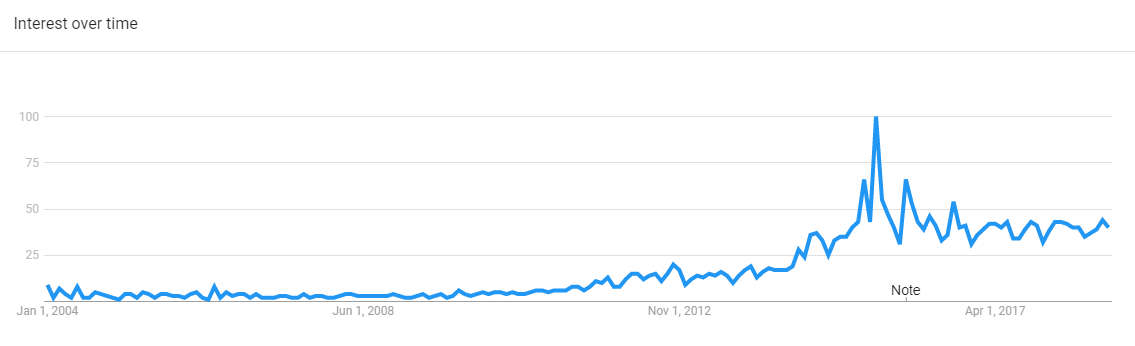
\includegraphics[width=1\textwidth]{figuras/chap-introduction/trends.png}
\caption{Evolution in the number of searches about the term Smart City in Google from 2004 to 2018}
\label{fig:trends}
\end{figure}

Besides tests and experiments of Smart Cities solutions, the simulator can also help city governments verifying the impacts of a myriad of actions in the city such as the building of a new bridge, of a new subway line, and changes in the bus lines itinerary. To evaluate the impact of these actions in the entire city, it is essential to provide a very-scalable simulator able to simulate the whole transportation infrastructure of the city, including the road network, subway network, and bus system. Most of the current open source and proprietary simulators can represent just a small area and with a limited number of agents. 
\section{Objectives and Challenges}
\label{sec:consideracoes_preliminares}

The primary objective of this work is design, implement, and evaluate the development of a large-scale Smart City simulator. The simulator must enable the simulation of a city with millions of actors in an extensive area such as the city of S\~ao Paulo with more than 11 million inhabitants, 4 million cars, 15 thousand buses, and 48 thousand streets in an area of more than 1,000 km\textsuperscript{2}. It is also objective of this work provide tools to facilitate the development of simulation scenarios using real data such as the map of the city, origin-destination surveys, and buses time-tables. The simulator also must generate output data that are easy to analyze and visualize.

A secondary objective is to show that the simulator is useful for different activities in Smart Cities projects. For example, the test and experiments of Smart City applications and platforms, to evaluate the infrastructure of a city, and as a testbed for new city simulation models.

To execute a simulation with the desired scalability, we had to solve many computational challenges. The first challenge was to select the right language and tools that enable the implementation of highly scalable software. Also, we had to test many data structures and algorithms to support the simulation scale. This research was necessary because most of the current simulators enable the simulation of just hundreds or thousands of simultaneous objects because of problems in their architecture. To simulate a city with the size of S\~ao Paulo in a reasonable time it is required a highly scalable and efficient implementation.

To achieve the necessary scalability, we developed a simulator able to execute parallel and distributed simulations. It adds yet more complexity to the implementation of the simulator because some of the models used in the simulator were never used in parallel implementations. To facilitate this task, we used Erlang, a language that promotes the development of scalable parallel and distributed applications. 

Finally, developing simulation models consistent with reality is also a challenge. To solve this problem, we made extensive research of different models and algorithms used to simulate cities such as traffic and public transportation models. We also used a lot of real-data such as maps and origin-destination surveys to further the realism of the simulations.

\section{Research Questions}

Our work involves answering the following three research questions:

\begin{description}
\item[RQ1:] ``What are the requirements to develop a general purpose, scalable Smart City simulator?''
\item[RQ2:] ``What is the most suitable programming model for the development of a large-scale Smart City simulator?''
\item[RQ3:] ``What are the possible uses of a large-scale Smart City simulator?''
\end{description}

To answer RQ1, we conducted a literature review of Smart Cities and related simulators. With this review, we identified the functional and non-functional requirements that a Smart City simulator should handle. For example, the simulator must represent the city map in an efficient data structure and allow a straightforward definition of the travels that must be simulated. 

To answer RQ2, we developed a Smart City simulator using Erlang, a language that implements the actor model and performed experiments to evaluate the simulator scalability. The evaluation shows that the simulator handles more than 20  millions actors efficiently in a single simulation executing faster than real-time.

Finally, to answer RQ3, we present the contexts that InterSCSimulator were already used and also describe other possible uses of the software. For example, the simulator was used to analyze the scalability of a Smart City platform and to compare mobility scenarios in the city of s\~ao Paulo.

\section{Thesis Organization}
\label{sec:organizacao_trabalho}

This thesis is organized as follows. Chapter \ref{cap:conceitos} presents the fundamental concepts used in this thesis which are Smart Cities, Traffic Simulation, and the Actor Model. Chapter \ref{cap:relacionados} cites related work including simulators of different domains of Smart Cities. Chapter \ref{cap:interscsimulator} introduces the development of InterSCSimulator, showing the functional and non-functional requirements, architecture, components, and implementation evolution. Chapter \ref{cap:sao_paulo} presents the simulation of the city of S\~ao Paulo, with more than 20 million travels, which served as the base for the scalability evaluation of the simulator. Chapter \ref{cap:avaliacao} presents the scalability evaluation of the simulator, showing experiments regarding its execution time and resources usage. Chapter \ref{cap:uses} presents examples of research already supported by the InterSCSimulator. Finally, Chapter \ref{cap:conclusoes} discusses the results of this thesis and future work.